\documentclass{beamer}

\usepackage{graphicx}
\usepackage{framed}

\begin{document}
	\begin{frame}
\begin{figure}
\centering

\includegraphics[width=0.7\linewidth]{plotlylogo}
\end{figure}
\end{frame}
%============================================%
\begin{frame}
\frametitle{plotly}
\large		
\begin{figure}
\centering
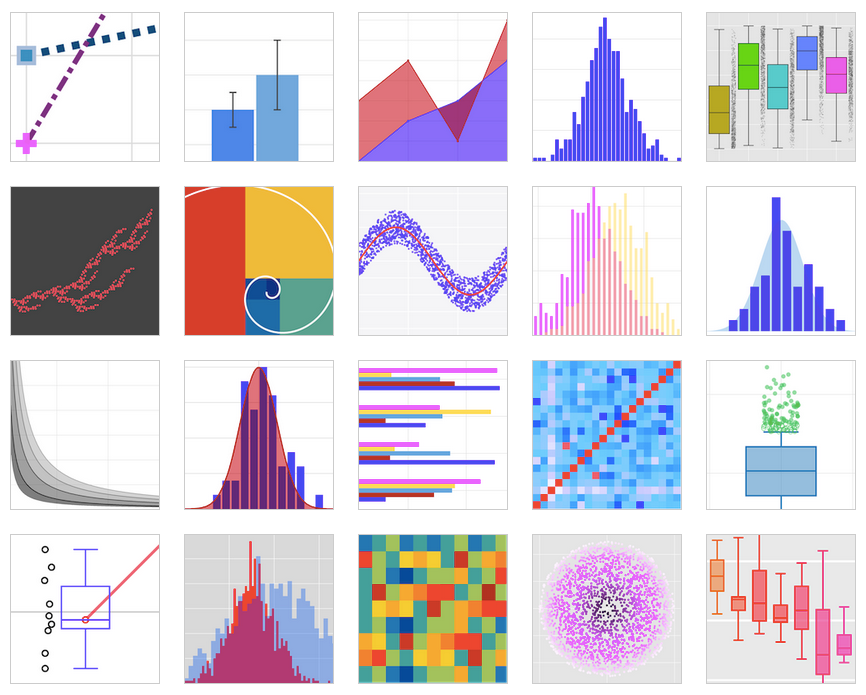
\includegraphics[width=0.7\linewidth]{plotlygallery}
\end{figure}

\end{frame}
%============================================%
\begin{frame}
\frametitle{plotly}
\Large	
About PlotLy
\begin{itemize}
	\item Plotly is the state of the art in data visualization, dashboards, and collaborative analysis, that can be used to make carts and dashboards.
\end{itemize}
\end{frame}

%==================================%
\begin{frame}
\frametitle{plotly}
\large	
\begin{itemize}
	\item Plotly's graphing libraries makes interactive, publication-quality graphs online, with libraries for Python, R, MATLAB, Perl, Julia, Arduino, and REST.
\end{itemize}
\end{frame}
%============================================%

\begin{frame}
	\large
	\texttt{Technology}
\begin{itemize}
	\item Plotly was built in Python and the Django framework, with a front end using JavaScript -- primarily the visualization library D3, HTML and CSS. 
	\item Files are hosted on Amazon S3. 
	\item Visualizations can't be viewed unless they're shared, Sundquist said, even if someone guesses the URL.
\end{itemize}

	
\end{frame}

%=============================================%
\begin{frame}[fragile]
	\large
\texttt{Installation}
\begin{framed}
\begin{verbatim}
pip install plotly
\end{verbatim}
\end{framed}
	\begin{figure}
\centering
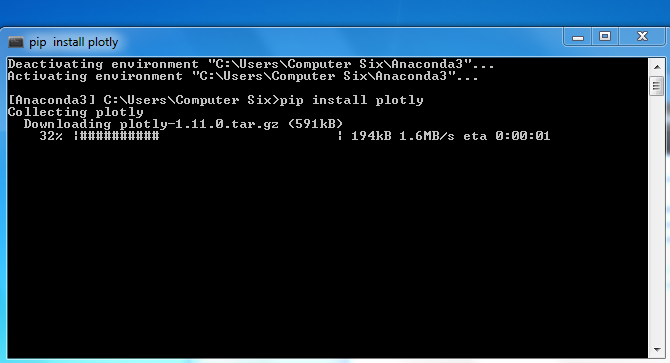
\includegraphics[width=0.95\linewidth]{pipinstallplotly}

\end{figure}

\end{frame}
%=============================================%
\begin{frame}
\large
\texttt{My PlotLy Account}
\begin{figure}
\centering
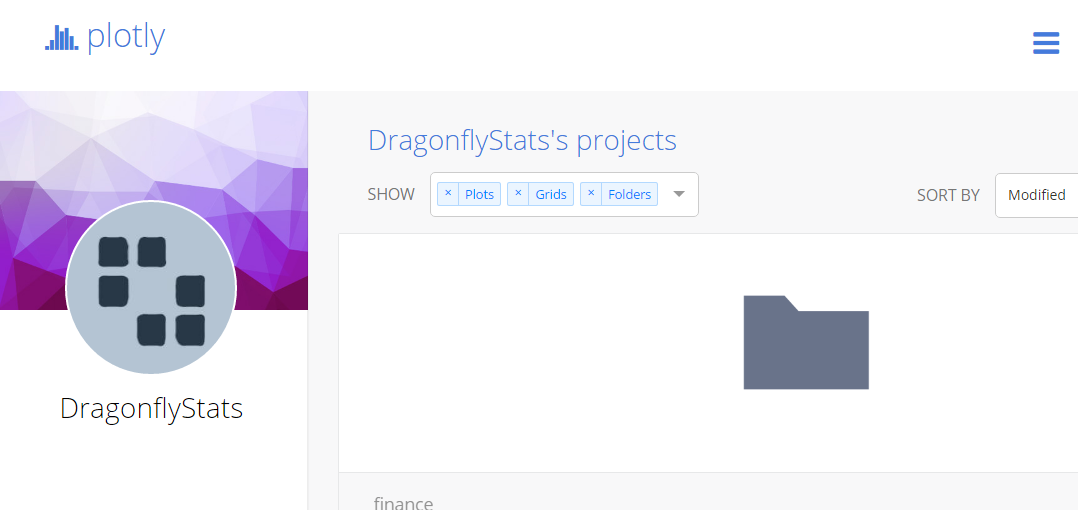
\includegraphics[width=01.1\linewidth]{plotlyprofile}
\end{figure}

\end{frame}
%=============================================%
\begin{frame}
	\large
	\texttt{Account Types}
	\begin{figure}
		\centering
		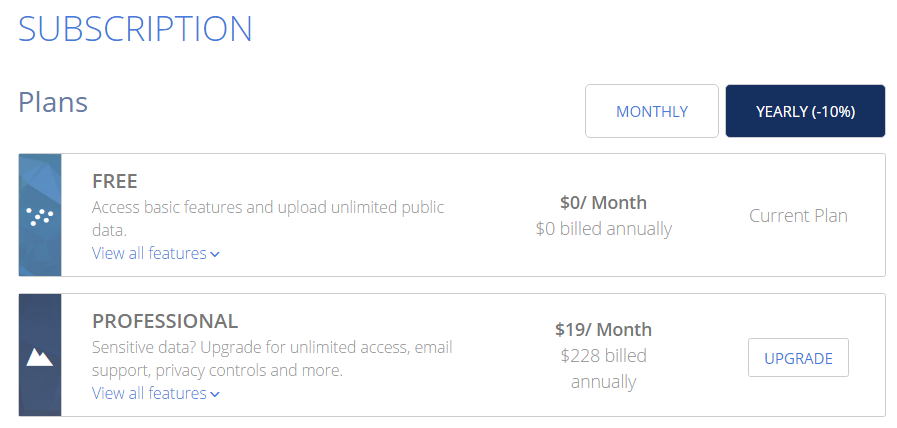
\includegraphics[width=01.1\linewidth]{plotlysubscription}
	\end{figure}
	
\end{frame}
%=============================================%
\begin{frame}
	\large
	\texttt{Industry}
	\begin{figure}
		\centering
		
\includegraphics[width=01.1\linewidth]{plotlyindustry}
	\end{figure}
	
\end{frame}


%==============================================%
\begin{frame}
	\begin{figure}
\centering

\includegraphics[width=1.3\linewidth]{jupyter}
\end{figure}
\end{frame}
%==============================================%
\end{document}
